\documentclass{beamer}
\usepackage{graphicx}
\usepackage[english]{babel}
\usepackage{hyperref}
\usepackage{multicol}
\usepackage{amssymb}
\usepackage{amsmath}

\usepackage{xcolor}
\usepackage{tikz}
\usetikzlibrary{calc}

\mode<presentation>
{ 
	\usetheme{Berkeley}
    \usecolortheme{default}
    \usefonttheme{structurebold}
}


% INCLUDE YOUR MENTORS ON YOUR FIRST SLIDE
\title[University of Michigan LoG(M)]{On the Statistics of Character Table of $S_n$}
\author{Tony Zhang}
\institute{University of Michigan}
\date{Last update \today}

\begin{document}
\begin{frame}
\titlepage
\end{frame}

\begin{frame}
\frametitle{Frobenius Formula}
\begin{theorem} [Frobenius Formula]
    \begin{itemize}
\item Given an integer partition $\lambda = \lambda_1 + \lambda_2 + \cdots + \lambda_k$ of $n$, let $\chi^{\lambda}$ be the corresponding irreducible character of $S_n$. 
\item Let $\chi^{\lambda}_{\mu}$ be short for the value of $\chi^{\lambda}$ at any $g$ with cycle type $\mu$, denote $l_j  =\lambda_j + k - j$, and $i_j$ the number of times $j$ appears in $\mu$, so $\sum\limits_j i_jj = n$
\item We have the following Frobenius Formula: 

 $\chi^{\lambda}_{\mu} = \text{coeff. of }  x_{1}^{l_1} x_{2}^{l_2}\cdots x_{k}^{l_k}$ in $\Delta(x) P_{\mu}(x)$
 
  
where $\Delta(x) = \prod\limits_{1 \leq i < j \leq k} (x_i-x_j)$, $P_\mu(x) = \prod\limits_j P_j(x_1,\cdots, x_k)^{i_j}$, where $P_j(x_1,\cdots, x_k) = x_1^j + \cdots + x_k^j$ is the $j$-th sum.
\end{itemize}
\end{theorem}
\end{frame}


\begin{frame}
\frametitle{Heatmap of character table for $n=20$}
\begin{figure}[H]
  \centering
  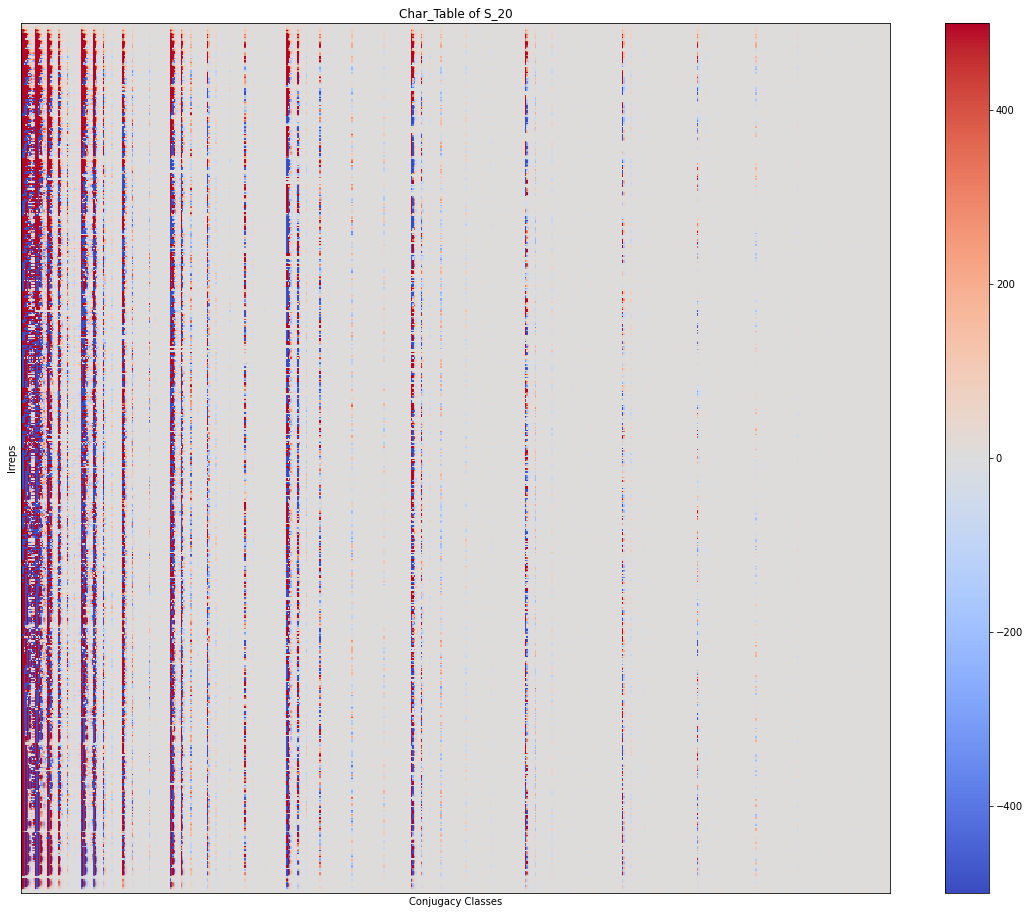
\includegraphics[width=0.6\linewidth]{char_table_20.png}
  \begin{center}
      \caption{\tiny Heatmap of Character Table for $n=20$ (values truncated within $\pm 500$)\footnote{ \tiny See the \href{https://github.com/TonyZhang2004/Character_Table_of_Symmetric_Groups/blob/main/char_table.ipynb}{\textcolor{blue}{program}}}}
  \end{center}
  
  \label{fig:char_20}
\end{figure}
\end{frame}

\begin{frame}
\frametitle{Heatmap of character table for $n=6$}

\begin{figure}[H]
  \centering
  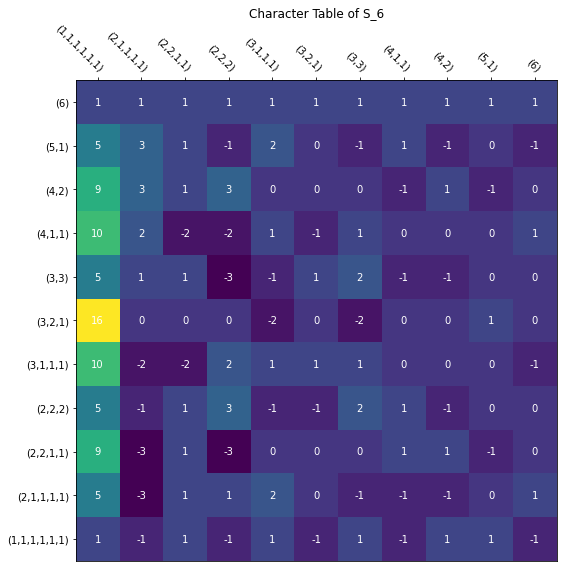
\includegraphics[width=0.4\linewidth]{char_table_6_heatmap.png}
  \caption{Heatmap of Character Table for $n=6$ 
 \footnote{ \tiny See the \href{https://github.com/TonyZhang2004/Character_Table_of_Symmetric_Groups/blob/main/char_table.ipynb}{\textcolor{blue}{program}}}}
  \label{fig:char_6}
\end{figure}

\begin{itemize}
	\item Rows are labeled with partitions corresponding to irreducible representations, columns are labeled with partitions corresponding to conjugacy classes.
\end{itemize}

\end{frame}
\iffalse
\begin{frame}
\frametitle{References}

\begin{thebibliography}{9}
\setbeamertemplate{bibliography item}[text]
\bibitem{Jane} Jane Doe. {\it A paper with theorems}. Preprint 2018.
\bibitem{logm} Lab of Geometry at Michigan. LoG(M) Beamer Template. {\em University of Michigan Department of Mathematics}. 2018.
\end{thebibliography}

\begin{center}
Special thanks to our mentors, first-names last-names!
\end{center}

\end{frame}
\fi
\end{document}

